
\begin{center}
    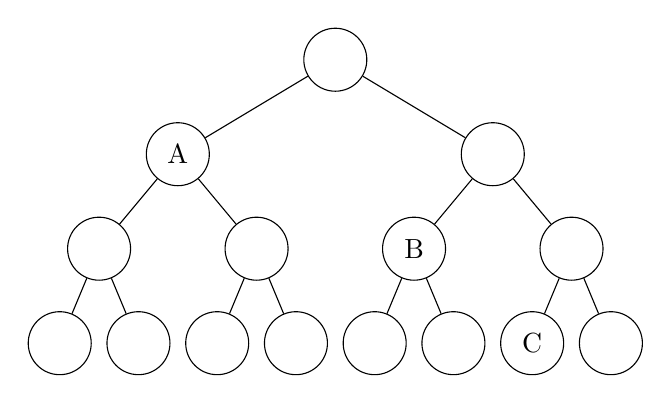
\begin{tikzpicture}[
      level distance=1.2cm,
      level 1/.style={sibling distance=4cm},
      level 2/.style={sibling distance=2cm},
      level 3/.style={sibling distance=1cm},
      every node/.style={draw,circle,minimum size=8mm,inner sep=1pt}
    ]
    
    % Root node with max value
    \node {}
        child {node {A}
            child {node {}
                child {node {}}
                child {node {}}
            }
            child {node {}
                child {node {}}
                child {node {}}
            }
        }
        child {node {}
            child {node {B}
                child {node {}}
                child {node {}}
            }
            child {node {}
                child {node {C}}
                child {node {}}
            }
        };
    
    \end{tikzpicture}
\end{center}